\section{分位数}
\label{sec:rvd-quantiles}

窗口想承诺“九成顾客的等待不超过某个时长”，这个时长应当定为多少？分布函数回答的是“给定阈值，累计概率多大”，现在的问题方向相反：给定累计概率$p$，求阈值$x$。

\paragraph{反解分布函数}
对等待时间，$F_T(t)=1-\mathrm{e}^{-t}$在$t\geq0$上连续且严格递增，方程$F_T(t)=p$对每个$0<p<1$恰有一个解：
\[
  1-\mathrm{e}^{-t}=p\quad\Longleftrightarrow\quad t=-\ln(1-p).
\]
取$p=0.9$，得$t=\ln10\approx2.303$分钟：九成顾客等待不超过约$2.3$分钟。

离散变量就没有这么顺利。公平骰子的分布函数在$[2,3)$上等于$1/3$，在$3$处跳到$1/2$，方程$F(x)=0.4$根本没有解；而$F(x)=1/2$对$[3,4)$中的每个$x$都成立，解有无穷多个。跳跃使某些$p$取不到，平台使某些$p$的解不唯一。我们需要一个对任何分布函数都有意义的约定。

自然的想法是不再要求“恰好等于$p$”，而是找累计概率首次达到$p$的位置。$p=0.4$时，阈值从左向右移动，到$x=3$时累计概率从$1/3$跳到$1/2$，第一次不小于$0.4$，所以取$3$。$p=1/2$时，累计概率在$x=3$处第一次达到$1/2$，平台上的其余点都在它右边，所以也取$3$。

\begin{definition}[分位数]
\label{def:rvd-quantile}
设$F$是随机变量$X$的分布函数，$0<p<1$。称
\begin{equation}
  Q(p)=\inf\{x\in\mathbb{R}:F(x)\geq p\}
  \label{eq:rvd-quantile}
\end{equation}
为$X$的$p$\term{分位数}（quantile），函数$p\mapsto Q(p)$称为\term{分位数函数}（quantile function）。$Q(1/2)$称为\term{中位数}（median），$Q(1/4)$与$Q(3/4)$分别称为下、上\term{四分位数}（quartile）。
\end{definition}

\paragraph{分位数与分布函数的对应}
分位数用到的只是分布函数的三条性质：单调不减、右连续、两端极限为$0$和$1$。前面各节的离散模型和密度模型都满足它们。下面的引理把下确界化成一个可以直接使用的等价关系。

\begin{lemma}[分位数的等价刻画]
\label{lem:rvd-quantile-galois}
设$0<p<1$。则$Q(p)$是有限实数，并且对一切实数$x$，
\begin{equation}
  Q(p)\leq x\quad\Longleftrightarrow\quad p\leq F(x).
  \label{eq:rvd-quantile-galois}
\end{equation}
\end{lemma}

\begin{proof}
记$A_p=\{x:F(x)\geq p\}$。因为$F(x)\to1>p$（$x\to+\infty$），$A_p$非空；因为$F(x)\to0<p$（$x\to-\infty$），$A_p$有下界。所以下确界$Q(p)$是有限实数。

$A_p$向右封闭：若$x\in A_p$且$y>x$，由单调性$F(y)\geq F(x)\geq p$，所以$y\in A_p$。再看下确界本身是否属于$A_p$。取$A_p$中的点列$x_n$从右侧趋于$Q(p)$，由右连续，
\[
  F(Q(p))=\lim_{n\to\infty}F(x_n)\geq p .
\]
所以$Q(p)\in A_p$，从而$A_p=[Q(p),\infty)$。“$x\in A_p$”就是“$p\leq F(x)$”，“$x\in[Q(p),\infty)$”就是“$Q(p)\leq x$”，二者等价。
\end{proof}

右连续在这里起了关键作用：它保证下确界被取到，集合$A_p$是带左端点的闭半直线。由引理可以读出分位数处的累计概率。取$x=Q(p)$，得$F(Q(p))\geq p$；对$x<Q(p)$有$F(x)<p$，令$x\uparrow Q(p)$，得左极限$F(Q(p)^{-})\leq p$。由式~\eqref{eq:rvd-jump}，这两条合起来是
\begin{equation}
  \mathbb{P}(X<Q(p))\leq p\leq\mathbb{P}(X\leq Q(p)).
  \label{eq:rvd-quantile-sandwich}
\end{equation}
也就是说，严格小于$p$分位数的概率至多是$p$，不超过它的概率至少是$p$。分布函数在$Q(p)$处连续时，两边相等，$F(Q(p))=p$。

\paragraph{平台与跳跃互换}
公平骰子的分位数函数可以直接写出。$F(x)=k/6$对$k\leq x<k+1$成立，由式~\eqref{eq:rvd-quantile-galois}，$Q(p)\leq k$当且仅当$p\leq k/6$，所以
\[
  Q(p)=k,\qquad \frac{k-1}{6}<p\leq\frac k6,\quad k=1,\dots,6 .
\]
特别地$Q(0.4)=3$，中位数$Q(1/2)=3$。图~\ref{fig:rvd-quantile-dice}把分布函数和分位数函数并排画出。

\begin{BookInlineFigure}
  \centering
  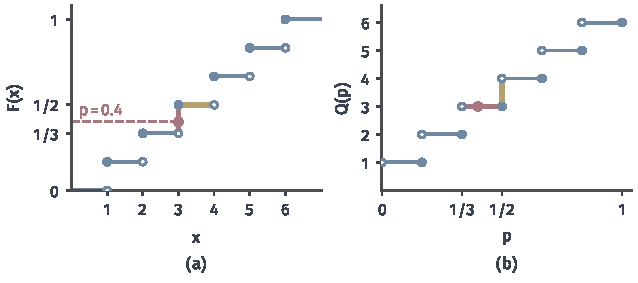
\includegraphics[width=108mm]{figures/07-probability/01-elementary-probability/matplotlib/rvd-quantile-dice/figure.pdf}
  \caption{公平骰子的分布函数与分位数函数。(a)分布函数，红色竖线是$x=3$处从$1/3$到$1/2$的跳跃，红色虚线$p=0.4$落在跳跃之内；黄线是高度$1/2$的平台$[3,4)$。(b)分位数函数，跳跃变成$(1/3,1/2]$上的平台（红线），红点是$Q(0.4)=3$；平台变成$p=1/2$处从$3$到$4$的跳跃（黄线）。实心点在每段右端，表示$Q$在跳跃点取左侧的值。}
  \label{fig:rvd-quantile-dice}
\end{BookInlineFigure}

图中可以看出两者的对偶。分布函数在$x=3$处跳跃$1/6$，累计概率在$(1/3,1/2]$中的所有$p$都“首次达到”于同一个位置$3$，于是分位数函数在这一段上是平台。分布函数在$[3,4)$上是平台，说明这一段没有质量，$p$稍大于$1/2$时阈值必须越过整段平台才能累计到更多概率，于是分位数函数在$p=1/2$处跳跃。几何上，分位数函数的图像就是把分布函数的图像沿对角线翻转，再在跳跃处按约定取左侧的值。

分位数函数单调不减，这由式~\eqref{eq:rvd-quantile}中集合$A_p$随$p$增大而缩小得到。它还是左连续的：设$p_n\uparrow p$，则$Q(p_n)$单调不减且不超过$Q(p)$，有极限$L\leq Q(p)$。对每个$n$有$Q(p_n)\leq L$，由引理$p_n\leq F(L)$；令$n\to\infty$得$p\leq F(L)$，再由引理$Q(p)\leq L$。所以$L=Q(p)$。分布函数右连续，分位数函数左连续，这是同一个约定的两面。

表~\ref{tab:rvd-cdf-vs-quantile}把两个函数的对应关系列在一起。

\begin{BookInlineTable}
  \centering
  \begin{tabular}{lll}
    \toprule
    & 分布函数$F$ & 分位数函数$Q$\\
    \midrule
    输入与输出 & 阈值$x\mapsto$累计概率 & 累计概率$p\mapsto$阈值\\
    定义域 & 全体实数 & $(0,1)$\\
    连续性约定 & 右连续 & 左连续\\
    跳跃 & 单点上的质量 & 一段没有质量的区间\\
    平台 & 一段没有质量的区间 & 单点上的质量\\
    \bottomrule
  \end{tabular}
  \caption{分布函数与分位数函数的对应。二者由式~\eqref{eq:rvd-quantile-galois}联系，一方的跳跃对应另一方的平台。}
  \label{tab:rvd-cdf-vs-quantile}
\end{BookInlineTable}

\paragraph{几个模型的分位数}
抽检次品数的分布函数是式~\eqref{eq:rvd-inspection-cdf}。用同样的方法读出
\[
  Q(p)=\begin{cases}0,&0<p\leq0.3,\\1,&0.3<p\leq0.9,\\2,&0.9<p<1.\end{cases}
\]
中位数是$1$：不超过$1$件次品的概率是$0.9$，严格少于$1$件的概率是$0.3$，两者把$1/2$夹在中间，与式~\eqref{eq:rvd-quantile-sandwich}一致。

等待时间的分位数函数是$Q(p)=-\ln(1-p)$。中位数和两个四分位数分别是
\[
  Q(\tfrac12)=\ln2\approx0.693,\quad Q(\tfrac14)=\ln\tfrac43\approx0.288,\quad Q(\tfrac34)=\ln4\approx1.386 .
\]
半数顾客等待不到$0.7$分钟，中间一半顾客的等待落在约$0.29$到$1.39$分钟之间。两个四分位数之差$Q(3/4)-Q(1/4)$称为\term{四分位距}（interquartile range），这里等于$\ln3\approx1.099$分钟，它从位置的角度衡量取值的分散程度。

另两个模型的分位数也有直接的含义。圆盘中随机点到圆心的距离满足$F_R(r)=r^{2}$，解得$Q(p)=\sqrt{p}$，中位数$\sqrt{1/2}\approx0.707$：一半的点落在半径约$0.707$的圆之外，因为这个圆的面积恰是整个圆盘的一半。

首次掷出六点所需的次数$N$满足$F_N(k)=1-(5/6)^{k}$。由式~\eqref{eq:rvd-quantile-galois}，$Q(p)\leq k$当且仅当$(5/6)^{k}\leq1-p$，即$k\geq\ln(1-p)/\ln(5/6)$，所以$Q(p)$是不小于$\ln(1-p)/\ln(5/6)$的最小正整数。算两个值：
\[
  F_N(3)=1-\tfrac{125}{216}\approx0.4213,\qquad F_N(4)=1-\tfrac{625}{1296}\approx0.5177 .
\]
累计概率在$k=4$时首次超过$1/2$，中位数是$4$。取$p=0.9$，$\ln0.1/\ln(5/6)\approx12.63$，于是$Q(0.9)=13$：要有九成把握见到六点，得准备掷$13$次。

\paragraph{平台上的中位数}
平台意味着一段没有质量的区间。设某服务只在两个时段开放，到达时刻$X$（单位：小时）在$[0,1]$与$[2,3]$上各以一半的概率均匀分布，即密度在这两段上为$1/2$，其余处为$0$。由式~\eqref{eq:rvd-cdf-from-density}，
\[
  F(x)=\begin{cases}x/2,&0\leq x\leq1,\\1/2,&1\leq x\leq2,\\(x-1)/2,&2\leq x\leq3,\end{cases}
\]
$x<0$时为$0$，$x>3$时为$1$。

图~\ref{fig:rvd-quantile-gap}显示，$F$在$[1,2]$上停在$1/2$。这一段的每个$m$都满足$\mathbb{P}(X\leq m)\geq1/2$且$\mathbb{P}(X\geq m)\geq1/2$，都把质量分成相等的两半。式~\eqref{eq:rvd-quantile}取其中最左的一个，$Q(1/2)=1$。也有书取平台的中点$1.5$，约定不同，但只有$F$在高度$p$处有平台时才会出现这种差别。

\begin{BookInlineFigure}
  \centering
  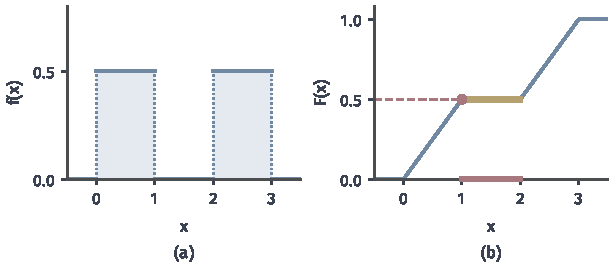
\includegraphics[width=104mm]{figures/07-probability/01-elementary-probability/matplotlib/rvd-quantile-gap/figure.pdf}
  \caption{密度有空档时的中位数。(a)密度在$[0,1]$与$[2,3]$上为$1/2$，中间为$0$；(b)分布函数在$[1,2]$上是高度$1/2$的平台（黄线），横轴上的红线$[1,2]$中每一点都把质量平分，红点是约定的中位数$Q(1/2)=1$。}
  \label{fig:rvd-quantile-gap}
\end{BookInlineFigure}

\paragraph{用二分法求分位数}
分布函数没有显式的反函数时，分位数要用数值方法求。引理~\ref{lem:rvd-quantile-galois}给出一个只用单调性的办法：对任意试探点$m$，计算$F(m)$并与$p$比较，$F(m)\geq p$说明$Q(p)\leq m$，否则$Q(p)>m$。每比较一次，就能把包含$Q(p)$的区间砍掉一半。这一判断不要求$F$连续或严格递增，跳跃和平台都不影响它。

以第~\ref{sec:rvd-mass-density}节的密度$6x(1-x)$为例，$F(x)=3x^{2}-2x^{3}$（$0\leq x\leq1$），求$0.9$分位数。中位数由对称性等于$1/2$，$0.9$分位数则要解三次方程$3x^{2}-2x^{3}=0.9$。从$[0,1]$出发，它一定包含$Q(0.9)$。每一轮取当前区间的中点$m$：若$F(m)\geq0.9$，把右端换成$m$；否则把左端换成$m$。前八轮的结果列在表~\ref{tab:rvd-bisection}中。

\begin{BookInlineTable}
  \centering
  \begin{tabular}{rllll}
    \toprule
    轮次 & 当前区间 & 中点$m$ & $F(m)$ & 判断\\
    \midrule
    1 & $[0,1]$ & $0.5$ & $0.5$ & $<0.9$，取右半\\
    2 & $[0.5,1]$ & $0.75$ & $0.8438$ & $<0.9$，取右半\\
    3 & $[0.75,1]$ & $0.875$ & $0.9570$ & $\geq0.9$，取左半\\
    4 & $[0.75,0.875]$ & $0.8125$ & $0.9077$ & $\geq0.9$，取左半\\
    5 & $[0.75,0.8125]$ & $0.78125$ & $0.8774$ & $<0.9$，取右半\\
    6 & $[0.78125,0.8125]$ & $0.796875$ & $0.8930$ & $<0.9$，取右半\\
    7 & $[0.796875,0.8125]$ & $0.8046875$ & $0.9005$ & $\geq0.9$，取左半\\
    8 & $[0.796875,0.8046875]$ & $0.80078125$ & $0.8967$ & $<0.9$，取右半\\
    \bottomrule
  \end{tabular}
  \caption{用二分法求$F(x)=3x^{2}-2x^{3}$的$0.9$分位数。每一轮区间长度减半，八轮后区间为$[0.80078125,0.8046875]$，长度$2^{-8}$。}
  \label{tab:rvd-bisection}
\end{BookInlineTable}

八轮之后，$Q(0.9)$被夹在$[0.80078,0.80469]$中，长度$2^{-8}\approx0.0039$。继续下去，区间收缩到$Q(0.9)\approx0.8042$。$k$轮之后区间长度是初始长度乘以$2^{-k}$，要达到精度$\varepsilon$只需约$\log_2(1/\varepsilon)$轮，每轮计算一次$F$。初始区间若未知，可以先向两侧加倍试探，直到找到$F(a)<p\leq F(b)$的两点。

\paragraph{分位数函数确定分布}
分位数函数是分布函数的广义逆，它是否也记下了全部信息？答案是肯定的，而且可以直接从引理~\ref{lem:rvd-quantile-galois}读出。对每个$x$，满足$Q(p)\leq x$的$p$恰是$(0,1)$中不超过$F(x)$的那些数，于是在$0<F(x)<1$时
\[
  F(x)=\max\{p\in(0,1):Q(p)\leq x\}.
\]
$F(x)=0$或$1$时，这个集合分别是空集或整个$(0,1)$，同样能读出$F(x)$。所以两个分布的分位数函数相同，它们的分布函数就相同。

还可以用分位数函数把一个最简单的随机变量变成任意给定分布的随机变量。设$U$有密度$1$（$0<u<1$），其余处为$0$，则$\mathbb{P}(U\leq u)=u$（$0\leq u\leq1$）。

\begin{theorem}[分位数变换]
\label{thm:rvd-quantile-transform}
设$F$是一个分布函数，$Q$是它的分位数函数，$U$如上。则$Q(U)$的分布函数是$F$。
\end{theorem}

\begin{proof}
$U$以概率$1$落在$(0,1)$中，那里$Q$有定义。对任意$x$，由引理~\ref{lem:rvd-quantile-galois}，$Q(U)\leq x$与$U\leq F(x)$是同一个事件，所以
\[
  \mathbb{P}(Q(U)\leq x)=\mathbb{P}(U\leq F(x))=F(x),
\]
最后一步用到$0\leq F(x)\leq1$。
\end{proof}

这个定理把“沿实轴均匀铺开的单位质量”按分位数函数重新安放：$U$落在$(1/3,1/2]$中的那一份质量，在骰子的例子中全部被送到$3$，于是$3$分到$1/6$的概率。

\paragraph{分位数与尾概率}
给定阈值$x$，事件$\{X>x\}$的概率$1-F(x)$称为$x$处的尾概率，它描述质量在$x$右侧的残余。给定小的比例$\alpha$，上侧分位数$Q(1-\alpha)$是“超过它的概率至多为$\alpha$”的最小阈值：由式~\eqref{eq:rvd-quantile-sandwich}，
\[
  \mathbb{P}\bigl(X>Q(1-\alpha)\bigr)=1-F\bigl(Q(1-\alpha)\bigr)\leq\alpha .
\]
尾概率和分位数是从两个方向读同一条曲线：前者由横轴读纵轴，后者由纵轴读横轴。

图~\ref{fig:rvd-quantile-tail}用等待时间演示。(a)从纵轴上的$0.5$和$0.9$出发读出中位数$\ln2$和$0.9$分位数$\ln10$。(b)画的是尾概率$1-F_T(t)=\mathrm{e}^{-t}$：从$t=1$读出$\mathbb{P}(T>1)=\mathrm{e}^{-1}\approx0.368$；在$t=\ln10$处尾概率恰为$0.1$，浅蓝面积就是这剩下的一成顾客。完整的分布已知时，两个方向都能精确计算；只知道分布的少数数值特征时，第~\ref{chap:tail-probabilities}章研究怎样给尾概率一个上界。

\begin{BookInlineFigure}
  \centering
  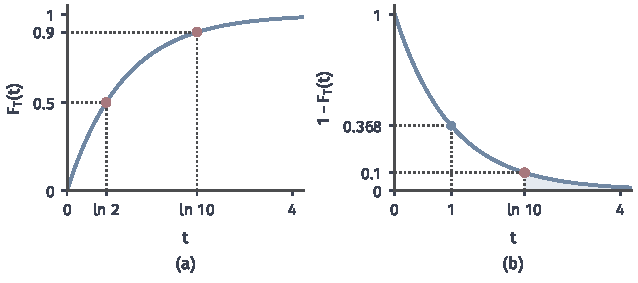
\includegraphics[width=108mm]{figures/07-probability/01-elementary-probability/matplotlib/rvd-quantile-tail/figure.pdf}
  \caption{等待时间的分位数与尾概率。(a)分布函数$1-\mathrm{e}^{-t}$，红点给出$Q(0.5)=\ln2$与$Q(0.9)=\ln10$；(b)尾概率$\mathrm{e}^{-t}$，蓝点是$t=1$处的$0.368$，红点是$t=\ln10$处的$0.1$，浅蓝区域表示超过$0.9$分位数的那部分。}
  \label{fig:rvd-quantile-tail}
\end{BookInlineFigure}

\paragraph{改变单位}
把等待时间从分钟换成秒，所有分位数都乘以$60$，这对一般的平移和正比例缩放都成立。设$a>0$，$b$为实数，$Y=aX+b$。对任意$y$，$\{Y\leq y\}=\{X\leq(y-b)/a\}$，所以$F_Y(y)=F_X((y-b)/a)$。由引理~\ref{lem:rvd-quantile-galois}，
\[
  Q_Y(p)\leq y\iff p\leq F_X\Bigl(\frac{y-b}{a}\Bigr)\iff Q_X(p)\leq\frac{y-b}{a}\iff aQ_X(p)+b\leq y .
\]
对一切$y$成立，于是$Q_Y(p)=aQ_X(p)+b$。$a<0$时不等号方向翻转，下侧分位数变成上侧，平台和跳跃处的约定也随之改变，需要另行处理。

\paragraph{描述位置而不是平均}
中位数和其他分位数描述的是分布的位置：取值在什么地方把质量按给定比例分开。它们只依赖取值的先后顺序和累计质量，不依赖远处的取值究竟有多远。

设$X$以概率$1/5$取$1,2,3,4,5$，中位数是$3$。把最大的取值$5$改成$12$，其余不变，$F$在$3$及其左侧不受影响，中位数仍是$3$。另一种描述中心的方式是按概率加权求和$\sum_xx\,p_X(x)$，下一章把它作为期望来研究。它同时看取值的大小，改动后从
\[
  \tfrac15(1+2+3+4+5)=3
\]
变为
\[
  \tfrac15(1+2+3+4+12)=4.4 .
\]
图~\ref{fig:rvd-median-shift}画出了这一对比：一个远处的取值就能把加权和拉过去，中位数却纹丝不动。

\begin{BookInlineFigure}
  \centering
  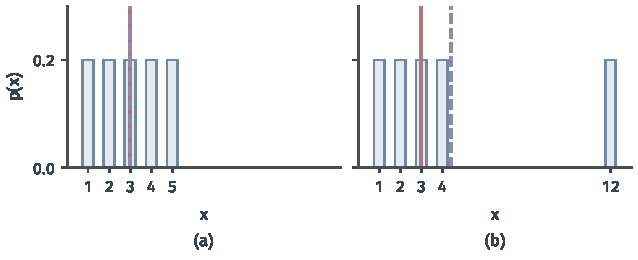
\includegraphics[width=108mm]{figures/07-probability/01-elementary-probability/matplotlib/rvd-median-shift/figure.pdf}
  \caption{中位数只看顺序。每个取值的概率都是$1/5$，红线是中位数$3$，紫色虚线是加权和$\sum_xx\,p_X(x)$。(a)取值$1,\dots,5$，两者都等于$3$；(b)把$5$移到$12$，中位数不变，加权和变为$4.4$。}
  \label{fig:rvd-median-shift}
\end{BookInlineFigure}

分位数还有一个优点：它对每个分布都存在。上一节的概率表$p_X(k)=1/(k(k+1))$有$F_X(1)=1/2$，所以中位数是$1$；而加权和
\[
  \sum_{k=1}^{\infty}k\cdot\frac{1}{k(k+1)}=\sum_{k=1}^{\infty}\frac{1}{k+1}
\]
是发散的调和级数，没有有限值。尾部质量衰减太慢时，加权平均会失去意义，分位数照样可以计算。至于什么时候加权平均存在、它与分位数各回答什么问题，在第~\ref{chap:random-variable-moments}章讨论。
